\documentclass[supplement,hidelinks]{siamart251216}
\usepackage{amssymb,mathtools}
\usepackage{booktabs}
\usepackage{array}
\usepackage{enumitem}
\usepackage[protrusion=true,expansion=false]{microtype}
\usepackage{placeins}
\graphicspath{{figures/}}
\usepackage{bm}
\usepackage{textcomp}
\renewcommand{\topfraction}{0.95}
\renewcommand{\bottomfraction}{0.9}
\renewcommand{\textfraction}{0.05}
\renewcommand{\floatpagefraction}{0.65}
\setlength{\emergencystretch}{1.5em}
\ifpdf
\hypersetup{
 pdftitle={Supplementary Materials: Symbol-based residual certification of reduced and neural surrogates for tempered-fractional CGMY pricing},
 pdfauthor={D. Damircheli}}
\fi
% Cross-references to the main article, frozen from its compiled .aux.
\newlabel{sec:introduction}{{1}{1}{Introduction}{}{}}
\newlabel{sec:introduction@cref}{{[section][1][]1}{[1][1][]1}}
\newlabel{sec:model}{{2}{2}{CGMY model and constrained discretisation}{}{}}
\newlabel{sec:model@cref}{{[section][2][]2}{[1][2][]2}}
\newlabel{sec:galerkin}{{2}{2}{CGMY model and constrained discretisation}{}{}}
\newlabel{sec:galerkin@cref}{{[section][2][]2}{[1][2][]2}}
\newlabel{ssec:operator}{{2.1}{2}{CGMY backward operator}{}{}}
\newlabel{ssec:operator@cref}{{[subsection][1][2]2.1}{[1][2][]2}}
\newlabel{eq:cgmy-parameters}{{2.1}{2}{CGMY backward operator}{}{}}
\newlabel{eq:cgmy-parameters@cref}{{[equation][1][2]2.1}{[1][2][]2}}
\newlabel{eq:martingale-correction}{{2.2}{2}{CGMY backward operator}{}{}}
\newlabel{eq:martingale-correction@cref}{{[equation][2][2]2.2}{[1][2][]2}}
\newlabel{eq:lambda0}{{2.3}{2}{CGMY backward operator}{}{}}
\newlabel{eq:lambda0@cref}{{[equation][3][2]2.3}{[1][2][]2}}
\newlabel{eq:tempered-ops}{{2.4}{3}{CGMY backward operator}{}{}}
\newlabel{eq:tempered-ops@cref}{{[equation][4][2]2.4}{[1][2][]3}}
\newlabel{eq:cgmy-operator}{{2.5}{3}{CGMY backward operator}{}{}}
\newlabel{eq:cgmy-operator@cref}{{[equation][5][2]2.5}{[1][3][]3}}
\newlabel{eq:pricing-pide}{{2.6}{3}{CGMY backward operator}{}{}}
\newlabel{eq:pricing-pide@cref}{{[equation][6][2]2.6}{[1][3][]3}}
\newlabel{eq:symbol}{{2.7}{3}{CGMY backward operator}{}{}}
\newlabel{eq:symbol@cref}{{[equation][7][2]2.7}{[1][3][]3}}
\newlabel{ssec:family}{{2.2}{3}{Parameter family and exterior data}{}{}}
\newlabel{ssec:family@cref}{{[subsection][2][2]2.2}{[1][3][]3}}
\newlabel{ssec:finite-domain}{{2.2}{3}{Parameter family and exterior data}{}{}}
\newlabel{ssec:finite-domain@cref}{{[subsection][2][2]2.2}{[1][3][]3}}
\newlabel{eq:parameter-set}{{2.8}{3}{Parameter family and exterior data}{}{}}
\newlabel{eq:parameter-set@cref}{{[equation][8][2]2.8}{[1][3][]3}}
\newlabel{eq:numerical-box}{{2.9}{3}{Parameter family and exterior data}{}{}}
\newlabel{eq:numerical-box@cref}{{[equation][9][2]2.9}{[1][3][]3}}
\newlabel{eq:energy-space}{{2.10}{3}{Parameter family and exterior data}{}{}}
\newlabel{eq:energy-space@cref}{{[equation][10][2]2.10}{[1][3][]3}}
\newlabel{eq:HMG-norm}{{2.11}{3}{Parameter family and exterior data}{}{}}
\newlabel{eq:HMG-norm@cref}{{[equation][11][2]2.11}{[1][3][]3}}
\newlabel{eq:weak-problem}{{2.12}{3}{Parameter family and exterior data}{}{}}
\newlabel{eq:weak-problem@cref}{{[equation][12][2]2.12}{[1][3][]3}}
\newlabel{eq:lifting-functional}{{2.13}{3}{Parameter family and exterior data}{}{}}
\newlabel{eq:lifting-functional@cref}{{[equation][13][2]2.13}{[1][3][]3}}
\newlabel{ssec:uniform}{{2.3}{4}{Uniform variational stability}{}{}}
\newlabel{ssec:uniform@cref}{{[subsection][3][2]2.3}{[1][3][]4}}
\newlabel{thm:uniform-coercivity}{{2.1}{4}{Uniform variational stability}{}{}}
\newlabel{thm:uniform-coercivity@cref}{{[theorem][1][2]2.1}{[1][4][]4}}
\newlabel{eq:uniform-coercivity}{{2.14}{4}{Uniform variational stability}{}{}}
\newlabel{eq:uniform-coercivity@cref}{{[equation][14][2]2.14}{[1][4][]4}}
\newlabel{rem:coercivity}{{2.2}{4}{Uniform variational stability}{}{}}
\newlabel{rem:coercivity@cref}{{[remark][2][2]2.2}{[1][4][]4}}
\newlabel{ssec:spline-space}{{2.4}{4}{Spline space and assembly}{}{}}
\newlabel{ssec:spline-space@cref}{{[subsection][4][2]2.4}{[1][4][]4}}
\newlabel{eq:Vh}{{2.15}{4}{Spline space and assembly}{}{}}
\newlabel{eq:Vh@cref}{{[equation][15][2]2.15}{[1][4][]4}}
\newlabel{eq:matrices}{{2.16}{4}{Spline space and assembly}{}{}}
\newlabel{eq:matrices@cref}{{[equation][16][2]2.16}{[1][4][]4}}
\newlabel{eq:Ah}{{2.17}{4}{Spline space and assembly}{}{}}
\newlabel{eq:Ah@cref}{{[equation][17][2]2.17}{[1][4][]4}}
\newlabel{eq:toeplitz-blocks}{{2.18}{4}{Spline space and assembly}{}{}}
\newlabel{eq:toeplitz-blocks@cref}{{[equation][18][2]2.18}{[1][4][]4}}
\newlabel{eq:semidiscrete-system}{{2.19}{4}{Spline space and assembly}{}{}}
\newlabel{eq:semidiscrete-system@cref}{{[equation][19][2]2.19}{[1][4][]4}}
\newlabel{ssec:assembly}{{2.5}{4}{Exact assembly from the periodised symbol}{}{}}
\newlabel{ssec:assembly@cref}{{[subsection][5][2]2.5}{[1][4][]4}}
\newlabel{lem:periodisation}{{2.3}{5}{Exact assembly from the periodised symbol}{}{}}
\newlabel{lem:periodisation@cref}{{[lemma][3][2]2.3}{[1][4][]5}}
\newlabel{eq:periodised}{{2.20}{5}{Exact assembly from the periodised symbol}{}{}}
\newlabel{eq:periodised@cref}{{[equation][20][2]2.20}{[1][4][]5}}
\newlabel{lem:tail}{{2.4}{5}{Exact assembly from the periodised symbol}{}{}}
\newlabel{lem:tail@cref}{{[lemma][4][2]2.4}{[1][5][]5}}
\newlabel{eq:tail}{{2.21}{5}{Exact assembly from the periodised symbol}{}{}}
\newlabel{eq:tail@cref}{{[equation][21][2]2.21}{[1][5][]5}}
\newlabel{lem:toeplitz}{{2.5}{6}{Exact assembly from the periodised symbol}{}{}}
\newlabel{lem:toeplitz@cref}{{[lemma][5][2]2.5}{[1][6][]6}}
\newlabel{ssec:constrained-system}{{2.6}{6}{Prescribed coefficients and the free system}{}{}}
\newlabel{ssec:constrained-system@cref}{{[subsection][6][2]2.6}{[1][6][]6}}
\newlabel{eq:constrained-cn}{{2.22}{6}{Prescribed coefficients and the free system}{}{}}
\newlabel{eq:constrained-cn@cref}{{[equation][22][2]2.22}{[1][6][]6}}
\newlabel{eq:constrained-residual}{{2.23}{6}{Prescribed coefficients and the free system}{}{}}
\newlabel{eq:constrained-residual@cref}{{[equation][23][2]2.23}{[1][6][]6}}
\newlabel{eq:sections}{{2.24}{6}{Prescribed coefficients and the free system}{}{}}
\newlabel{eq:sections@cref}{{[equation][24][2]2.24}{[1][6][]6}}
\newlabel{ssec:reference-time}{{2.7}{7}{Time discretisation and error target}{}{}}
\newlabel{ssec:reference-time@cref}{{[subsection][7][2]2.7}{[1][7][]7}}
\newlabel{ssec:deterministic-error}{{2.7}{7}{Time discretisation and error target}{}{}}
\newlabel{ssec:deterministic-error@cref}{{[subsection][7][2]2.7}{[1][7][]7}}
\newlabel{ssec:lifting-cancels}{{2.7}{7}{Time discretisation and error target}{}{}}
\newlabel{ssec:lifting-cancels@cref}{{[subsection][7][2]2.7}{[1][7][]7}}
\newlabel{eq:cn-reference}{{2.25}{7}{Time discretisation and error target}{}{}}
\newlabel{eq:cn-reference@cref}{{[equation][25][2]2.25}{[1][7][]7}}
\newlabel{eq:total-error-split}{{2.26}{7}{Time discretisation and error target}{}{}}
\newlabel{eq:total-error-split@cref}{{[equation][26][2]2.26}{[1][7][]7}}
\newlabel{ssec:spectral}{{2.8}{7}{Spectral lower bound}{}{}}
\newlabel{ssec:spectral@cref}{{[subsection][8][2]2.8}{[1][7][]7}}
\newlabel{lem:LK}{{2.6}{7}{Spectral lower bound}{}{}}
\newlabel{lem:LK@cref}{{[lemma][6][2]2.6}{[1][7][]7}}
\newlabel{thm:spectral}{{2.7}{7}{Spectral lower bound}{}{}}
\newlabel{thm:spectral@cref}{{[theorem][7][2]2.7}{[1][7][]7}}
\newlabel{eq:spectral}{{2.27}{7}{Spectral lower bound}{}{}}
\newlabel{eq:spectral@cref}{{[equation][27][2]2.27}{[1][7][]7}}
\newlabel{rem:compression}{{2.8}{8}{Spectral lower bound}{}{}}
\newlabel{rem:compression@cref}{{[remark][8][2]2.8}{[1][7][]8}}
\newlabel{sec:certificate}{{3}{8}{Residual certification and tolerance-controlled correction}{}{}}
\newlabel{sec:certificate@cref}{{[section][3][]3}{[1][8][]8}}
\newlabel{sec:pcc}{{3}{8}{Residual certification and tolerance-controlled correction}{}{}}
\newlabel{sec:pcc@cref}{{[section][3][]3}{[1][8][]8}}
\newlabel{ssec:riesz}{{3.1}{8}{Energy norm and Crank--Nicolson bound}{}{}}
\newlabel{ssec:riesz@cref}{{[subsection][1][3]3.1}{[1][8][]8}}
\newlabel{ssec:cn-certificate}{{3.1}{8}{Energy norm and Crank--Nicolson bound}{}{}}
\newlabel{ssec:cn-certificate@cref}{{[subsection][1][3]3.1}{[1][8][]8}}
\newlabel{eq:Sh}{{3.1}{8}{Energy norm and Crank--Nicolson bound}{}{}}
\newlabel{eq:Sh@cref}{{[equation][1][3]3.1}{[1][8][]8}}
\newlabel{eq:cn-residual}{{3.2}{8}{Energy norm and Crank--Nicolson bound}{}{}}
\newlabel{eq:cn-residual@cref}{{[equation][2][3]3.2}{[1][8][]8}}
\newlabel{eq:discrete-error-equation}{{3.3}{8}{Energy norm and Crank--Nicolson bound}{}{}}
\newlabel{eq:discrete-error-equation@cref}{{[equation][3][3]3.3}{[1][8][]8}}
\newlabel{thm:fully-discrete-certificate}{{3.1}{8}{Energy norm and Crank--Nicolson bound}{}{}}
\newlabel{thm:fully-discrete-certificate@cref}{{[theorem][1][3]3.1}{[1][8][]8}}
\newlabel{eq:fully-discrete-certificate}{{3.4}{8}{Energy norm and Crank--Nicolson bound}{}{}}
\newlabel{eq:fully-discrete-certificate@cref}{{[equation][4][3]3.4}{[1][8][]8}}
\newlabel{eq:sharp-estimator}{{3.5}{9}{Energy norm and Crank--Nicolson bound}{}{}}
\newlabel{eq:sharp-estimator@cref}{{[equation][5][3]3.5}{[1][8][]9}}
\newlabel{eq:sharp-L2}{{3.6}{9}{Energy norm and Crank--Nicolson bound}{}{}}
\newlabel{eq:sharp-L2@cref}{{[equation][6][3]3.6}{[1][9][]9}}
\newlabel{ssec:guaranteed}{{3.2}{9}{Upper bounds from incomplete Riesz solves}{}{}}
\newlabel{ssec:guaranteed@cref}{{[subsection][2][3]3.2}{[1][9][]9}}
\newlabel{eq:alpha-lb}{{3.7}{9}{Upper bounds from incomplete Riesz solves}{}{}}
\newlabel{eq:alpha-lb@cref}{{[equation][7][3]3.7}{[1][9][]9}}
\newlabel{lem:guaranteed}{{3.2}{9}{Upper bounds from incomplete Riesz solves}{}{}}
\newlabel{lem:guaranteed@cref}{{[lemma][2][3]3.2}{[1][9][]9}}
\newlabel{eq:riesz-bracket-def}{{3.8}{9}{Upper bounds from incomplete Riesz solves}{}{}}
\newlabel{eq:riesz-bracket-def@cref}{{[equation][8][3]3.8}{[1][9][]9}}
\newlabel{cor:guaranteed}{{3.3}{9}{Upper bounds from incomplete Riesz solves}{}{}}
\newlabel{cor:guaranteed@cref}{{[corollary][3][3]3.3}{[1][9][]9}}
\newlabel{eq:guaranteed-estimator}{{3.9}{9}{Upper bounds from incomplete Riesz solves}{}{}}
\newlabel{eq:guaranteed-estimator@cref}{{[equation][9][3]3.9}{[1][9][]9}}
\newlabel{rem:arithmetic-scope}{{3.4}{10}{Upper bounds from incomplete Riesz solves}{}{}}
\newlabel{rem:arithmetic-scope@cref}{{[remark][4][3]3.4}{[1][10][]10}}
\newlabel{ssec:comparison}{{3.3}{10}{A banded comparison norm}{}{}}
\newlabel{ssec:comparison@cref}{{[subsection][3][3]3.3}{[1][10][]10}}
\newlabel{thm:comparison}{{3.5}{10}{A banded comparison norm}{}{}}
\newlabel{thm:comparison@cref}{{[theorem][5][3]3.5}{[1][10][]10}}
\newlabel{eq:comparison}{{3.10}{10}{A banded comparison norm}{}{}}
\newlabel{eq:comparison@cref}{{[equation][10][3]3.10}{[1][10][]10}}
\newlabel{cor:cheap}{{3.6}{10}{A banded comparison norm}{}{}}
\newlabel{cor:cheap@cref}{{[corollary][6][3]3.6}{[1][10][]10}}
\newlabel{prop:twostage}{{3.7}{10}{A banded comparison norm}{}{}}
\newlabel{prop:twostage@cref}{{[proposition][7][3]3.7}{[1][10][]10}}
\newlabel{prop:threestage}{{3.8}{11}{A banded comparison norm}{}{}}
\newlabel{prop:threestage@cref}{{[proposition][8][3]3.8}{[1][11][]11}}
\newlabel{ssec:efficiency}{{3.4}{11}{Efficiency and spot-price bounds}{}{}}
\newlabel{ssec:efficiency@cref}{{[subsection][4][3]3.4}{[1][11][]11}}
\newlabel{ssec:greeks-cert}{{3.4}{11}{Efficiency and spot-price bounds}{}{}}
\newlabel{ssec:greeks-cert@cref}{{[subsection][4][3]3.4}{[1][11][]11}}
\newlabel{eq:kappa-def}{{3.11}{11}{Efficiency and spot-price bounds}{}{}}
\newlabel{eq:kappa-def@cref}{{[equation][11][3]3.11}{[1][11][]11}}
\newlabel{thm:efficiency}{{3.9}{11}{Efficiency and spot-price bounds}{}{}}
\newlabel{thm:efficiency@cref}{{[theorem][9][3]3.9}{[1][11][]11}}
\newlabel{eq:efficiency}{{3.12}{12}{Efficiency and spot-price bounds}{}{}}
\newlabel{eq:efficiency@cref}{{[equation][12][3]3.12}{[1][11][]12}}
\newlabel{eq:gamma-infty}{{3.13}{12}{Efficiency and spot-price bounds}{}{}}
\newlabel{eq:gamma-infty@cref}{{[equation][13][3]3.13}{[1][12][]12}}
\newlabel{ssec:algorithm}{{3.5}{12}{Tolerance-controlled prediction and correction}{}{}}
\newlabel{ssec:algorithm@cref}{{[subsection][5][3]3.5}{[1][12][]12}}
\newlabel{ssec:two-stage}{{3.5}{12}{Tolerance-controlled prediction and correction}{}{}}
\newlabel{ssec:two-stage@cref}{{[subsection][5][3]3.5}{[1][12][]12}}
\newlabel{ssec:correction}{{3.5}{12}{Tolerance-controlled prediction and correction}{}{}}
\newlabel{ssec:correction@cref}{{[subsection][5][3]3.5}{[1][12][]12}}
\newlabel{alg:pcc}{{3.1}{12}{Tolerance-checked online rule (the three-stage rule of Proposition~\ref {prop:threestage} followed by correction). The status names are those used in the tables of Section~\ref {sec:numerics}}{}{}}
\newlabel{alg:pcc@cref}{{[figure][1][3]3.1}{[1][12][]12}}
\newlabel{prop:two-stage}{{3.10}{12}{Tolerance-controlled prediction and correction}{}{}}
\newlabel{prop:two-stage@cref}{{[proposition][10][3]3.10}{[1][12][]12}}
\newlabel{eq:soundness}{{3.14}{12}{Tolerance-controlled prediction and correction}{}{}}
\newlabel{eq:soundness@cref}{{[equation][14][3]3.14}{[1][12][]12}}
\newlabel{eq:correction-step}{{3.15}{13}{Tolerance-controlled prediction and correction}{}{}}
\newlabel{eq:correction-step@cref}{{[equation][15][3]3.15}{[1][13][]13}}
\newlabel{sec:affine}{{4}{13}{Affine structure and surrogate candidates}{}{}}
\newlabel{sec:affine@cref}{{[section][4][]4}{[1][13][]13}}
\newlabel{sec:operator}{{4}{13}{Affine structure and surrogate candidates}{}{}}
\newlabel{sec:operator@cref}{{[section][4][]4}{[1][13][]13}}
\newlabel{ssec:eim}{{4.1}{13}{Affine decomposition of the fractional blocks}{}{}}
\newlabel{ssec:eim@cref}{{[subsection][1][4]4.1}{[1][13][]13}}
\newlabel{eq:affine-split}{{4.1}{13}{Affine decomposition of the fractional blocks}{}{}}
\newlabel{eq:affine-split@cref}{{[equation][1][4]4.1}{[1][13][]13}}
\newlabel{lem:eim}{{4.1}{13}{Affine decomposition of the fractional blocks}{}{}}
\newlabel{lem:eim@cref}{{[lemma][1][4]4.1}{[1][13][]13}}
\newlabel{fig:eim}{{4.1}{14}{Empirical interpolation of the fractional symbol family. (a) Relative sup-norm error on $1000$ Sobol test parameters (solid) and normalised singular values of the $16^3$ training snapshots (dotted), $N=64$--$1024$. (b) Rank $Q$ needed for a given test tolerance; the curves for $N=512$ and $N=1024$ coincide. The operational $Q$ additionally satisfies the operator-norm check (one extra term at $N=64$)}{}{}}
\newlabel{fig:eim@cref}{{[figure][1][4]4.1}{[1][13][]14}}
\newlabel{thm:eim-cert}{{4.2}{14}{Affine decomposition of the fractional blocks}{}{}}
\newlabel{thm:eim-cert@cref}{{[theorem][2][4]4.2}{[1][14][]14}}
\newlabel{rem:reduced-online}{{4.3}{15}{Affine decomposition of the fractional blocks}{}{}}
\newlabel{rem:reduced-online@cref}{{[remark][3][4]4.3}{[1][15][]15}}
\newlabel{ssec:target}{{4.2}{15}{Candidates, initial target and training objective}{}{}}
\newlabel{ssec:target@cref}{{[subsection][2][4]4.2}{[1][15][]15}}
\newlabel{ssec:architectures}{{4.2}{15}{Candidates, initial target and training objective}{}{}}
\newlabel{ssec:architectures@cref}{{[subsection][2][4]4.2}{[1][15][]15}}
\newlabel{ssec:exact-ic}{{4.2}{15}{Candidates, initial target and training objective}{}{}}
\newlabel{ssec:exact-ic@cref}{{[subsection][2][4]4.2}{[1][15][]15}}
\newlabel{ssec:losses}{{4.2}{15}{Candidates, initial target and training objective}{}{}}
\newlabel{ssec:losses@cref}{{[subsection][2][4]4.2}{[1][15][]15}}
\newlabel{sec:data}{{4.2}{15}{Candidates, initial target and training objective}{}{}}
\newlabel{sec:data@cref}{{[subsection][2][4]4.2}{[1][15][]15}}
\newlabel{eq:residual-loss}{{4.2}{15}{Candidates, initial target and training objective}{}{}}
\newlabel{eq:residual-loss@cref}{{[equation][2][4]4.2}{[1][15][]15}}
\newlabel{ssec:pod-construction}{{4.3}{16}{Mass-weighted POD trajectories}{}{}}
\newlabel{ssec:pod-construction@cref}{{[subsection][3][4]4.3}{[1][16][]16}}
\newlabel{eq:repaired-pod-cn}{{4.3}{16}{Mass-weighted POD trajectories}{}{}}
\newlabel{eq:repaired-pod-cn@cref}{{[equation][3][4]4.3}{[1][16][]16}}
\newlabel{ssec:cost}{{4.4}{17}{Cost model}{}{}}
\newlabel{ssec:cost@cref}{{[subsection][4][4]4.4}{[1][17][]17}}
\newlabel{sec:numerics}{{5}{17}{Numerical evaluation}{}{}}
\newlabel{sec:numerics@cref}{{[section][5][]5}{[1][17][]17}}
\newlabel{ssec:design}{{5.1}{17}{Experimental design}{}{}}
\newlabel{ssec:design@cref}{{[subsection][1][5]5.1}{[1][17][]17}}
\newlabel{tab:populations}{{5.1}{17}{Experimental design}{}{}}
\newlabel{tab:populations@cref}{{[subsection][1][5]5.1}{[1][17][]17}}
\newlabel{ssec:verification}{{5.2}{17}{Verification of the assembly, the bounds and the solvers}{}{}}
\newlabel{ssec:verification@cref}{{[subsection][2][5]5.2}{[1][17][]17}}
\newlabel{ssec:e0-assembly}{{5.2}{17}{Verification of the assembly, the bounds and the solvers}{}{}}
\newlabel{ssec:e0-assembly@cref}{{[subsection][2][5]5.2}{[1][17][]17}}
\newlabel{ssec:e0-spectral}{{5.2}{17}{Verification of the assembly, the bounds and the solvers}{}{}}
\newlabel{ssec:e0-spectral@cref}{{[subsection][2][5]5.2}{[1][17][]17}}
\newlabel{ssec:e0-riesz}{{5.2}{17}{Verification of the assembly, the bounds and the solvers}{}{}}
\newlabel{ssec:e0-riesz@cref}{{[subsection][2][5]5.2}{[1][17][]17}}
\newlabel{ssec:e0-initial}{{5.2}{17}{Verification of the assembly, the bounds and the solvers}{}{}}
\newlabel{ssec:e0-initial@cref}{{[subsection][2][5]5.2}{[1][17][]17}}
\newlabel{ssec:calibration}{{5.3}{18}{Resolution and tolerance calibration}{}{}}
\newlabel{ssec:calibration@cref}{{[subsection][3][5]5.3}{[1][18][]18}}
\newlabel{tab:budget}{{5.1}{18}{Resolution and tolerance calibration: maximum price error $\max |V_h(T,S)-V_{\mathrm {COS}}|$ over the 30 price-diagnostic queries and the two box corners, spots $S\in \{0.8,\dots ,1.2\}\mathcal K$; COS with 8192 modes, range parameter 30. $\varepsilon _N=\tau _\$/\max _s\beta _I(x_s)$ with $\tau _\$=1$ cent}{}{}}
\newlabel{tab:budget@cref}{{[table][1][5]5.1}{[1][18][]18}}
\newlabel{ssec:e1}{{5.4}{18}{Reduced model and neural candidates}{}{}}
\newlabel{ssec:e1@cref}{{[subsection][4][5]5.4}{[1][18][]18}}
\newlabel{ssec:pod-results}{{5.4}{18}{Reduced model and neural candidates}{}{}}
\newlabel{ssec:pod-results@cref}{{[subsection][4][5]5.4}{[1][18][]18}}
\newlabel{tab:pod-ranks}{{5.2}{19}{POD--Galerkin candidates on the 30 validation queries at the production configuration ($N=1024$, $N_T=240$, $Q$ matched to $\varepsilon $): median maximum-in-time mass-norm error against the direct solution, median effectivity (bound/error) of the three certificates, queries accepted at $\varepsilon _N=1.18\times 10^{-3}$ under each certificate, and the stage at which the three-stage rule of Proposition~\ref {prop:threestage} settles the query (reduced accept / cheap reject / banded accept / exact accept / exact reject). Basis from 800 training trajectories; the 4000-trajectory basis gives the same picture (Section~\ref {ssec:e1}). No false accepts occur under any certificate at any tolerance of the sweep}{}{}}
\newlabel{tab:pod-ranks@cref}{{[table][2][5]5.2}{[1][18][]19}}
\newlabel{fig:acceptance}{{5.1}{19}{Top: accepted fraction of the 30 validation queries as a function of the tolerance $\varepsilon $ (dashed line: $\varepsilon _N$) for POD--Galerkin candidates of rank $48$--$80$ and the two best POD-NN checkpoints, under the reduced online, banded full-order and exact full-order certificates. Bottom: the stage at which the three-stage rule of Proposition~\ref {prop:threestage} settles each query at $\varepsilon _N$, per rank}{}{}}
\newlabel{fig:acceptance@cref}{{[figure][1][5]5.1}{[1][18][]19}}
\newlabel{ssec:benchmark}{{5.5}{20}{Matched benchmark and cost under refinement}{}{}}
\newlabel{ssec:benchmark@cref}{{[subsection][5][5]5.5}{[1][20][]20}}
\newlabel{ssec:scaling-results}{{5.5}{20}{Matched benchmark and cost under refinement}{}{}}
\newlabel{ssec:scaling-results@cref}{{[subsection][5][5]5.5}{[1][20][]20}}
\newlabel{ssec:ood}{{5.6}{20}{Out-of-distribution detection}{}{}}
\newlabel{ssec:ood@cref}{{[subsection][6][5]5.6}{[1][20][]20}}
\newlabel{fig:benchmark}{{5.2}{21}{Top: time ratio to the uncertified direct solve on the 120 benchmark queries at $\varepsilon =0.3\varepsilon _N$, $\varepsilon _N$, $3\varepsilon _N$ (geometric means, $95\%$ query-bootstrap intervals, reusable setup). Bottom left: direct solve and banded full-order certificate per query as functions of $N$ (20 benchmark queries, $N_T=240$), with the reduced online certificate at $r=64$ and $80$, which does not depend on $N$. Bottom right: the certificate as a fraction of the solve, $4.5$--$5.6\%$ for $N=64$--$4096$}{}{}}
\newlabel{fig:benchmark@cref}{{[figure][2][5]5.2}{[1][20][]21}}
\newlabel{tab:benchmark}{{5.3}{21}{Matched benchmark on the 120 benchmark queries at the production configuration (one thread, idle machine, reusable setup, five repetitions): geometric-mean time ratio to the uncertified direct solve with 95\% query-bootstrap interval, three-stage outcome (reduced accept / cheap reject / banded or exact accept / corrected), and false accepts. The direct solve takes $259$~ms; the certificate proper is $6.0\%$ of it and $7.2\%$ with the per-query spectral data}{}{}}
\newlabel{tab:benchmark@cref}{{[table][3][5]5.3}{[1][20][]21}}
\newlabel{tab:ood}{{5.4}{22}{Out-of-distribution study: 264 queries outside the parameter box (200 Sobol points in the shells $C\in [1,2]$, $Y\in [0.9,1.1)\cup (1.8,1.95]$, $G\in [0.5,1)$, $M\in [9,15]$, and 64 vertices of the extended box) at the production configuration. Top: queries on which the candidate's true error is below $\varepsilon _N$ (``works''), queries the exact certificate accepts (``certified''), and precision of two rules as detectors of ``true error $>\varepsilon _N$'': the certificate (recall 1 by theorem) and the naive rule that rejects every query outside the training box (recall 1, but it discards every working query). Bottom: POD--Galerkin $r=80$ by shell (a query leaving the box in several coordinates counts in each), with the median true error and the median EIM error $\varepsilon _Q$ (inside the box: $1.7\times 10^{-9}$)}{}{}}
\newlabel{tab:ood@cref}{{[table][4][5]5.4}{[1][21][]22}}
\newlabel{fig:ood}{{5.3}{22}{Certified bound against true error for the 264 out-of-box queries and the 30 validation queries (POD--Galerkin $r=64$ and $80$, space--time POD-NN), under the three certificates; the lines mark $\varepsilon _N$ and bound $=$ error}{}{}}
\newlabel{fig:ood@cref}{{[figure][3][5]5.3}{[1][21][]22}}
\newlabel{ssec:multiquery}{{5.7}{22}{Multi-query cost and amortisation}{}{}}
\newlabel{ssec:multiquery@cref}{{[subsection][7][5]5.7}{[1][22][]22}}
\newlabel{fig:online-time}{{5.4}{23}{Online time per query of the reduced model at the production configuration (one thread, idle machine): reduced solve, reduced online certificate, and the three-stage total at $\varepsilon _N$, against the uncertified direct solve (dashed: cold-start and reusable-setup medians of the benchmark of Section~\ref {ssec:benchmark})}{}{}}
\newlabel{fig:online-time@cref}{{[figure][4][5]5.4}{[1][22][]23}}
\newlabel{fig:amortisation}{{5.5}{23}{Cumulative wall time, offline cost included, against the number of queries at the production configuration (one thread); dots mark the break-even with the uncertified direct solver}{}{}}
\newlabel{fig:amortisation@cref}{{[figure][5][5]5.5}{[1][22][]23}}
\newlabel{ssec:archive}{{5.8}{23}{Reproducibility}{}{}}
\newlabel{ssec:archive@cref}{{[subsection][8][5]5.8}{[1][23][]23}}
\newlabel{sec:conclusion}{{6}{23}{Conclusion}{}{}}
\newlabel{sec:conclusion@cref}{{[section][6][]6}{[1][23][]23}}
\newlabel{sec:discussion}{{6}{23}{Conclusion}{}{}}
\newlabel{sec:discussion@cref}{{[section][6][]6}{[1][23][]23}}
\newlabel{app:proofs}{{A}{24}{Conclusion}{}{}}
\newlabel{app:proofs@cref}{{[appendix][1][2147483647]A}{[1][24][]24}}
\newlabel{app:proof-uniform}{{A.1}{24}{Proof of Theorem~\ref {thm:uniform-coercivity}}{}{}}
\newlabel{app:proof-uniform@cref}{{[subappendix][1][2147483647,1]A.1}{[1][24][]24}}
\newlabel{ssec:lk-coercivity}{{A.1}{24}{Proof of Theorem~\ref {thm:uniform-coercivity}}{}{}}
\newlabel{ssec:lk-coercivity@cref}{{[subappendix][1][2147483647,1]A.1}{[1][24][]24}}
\newlabel{eq:c1-explicit}{{A.1}{24}{Proof of Theorem~\ref {thm:uniform-coercivity}}{}{}}
\newlabel{eq:c1-explicit@cref}{{[equation][1][2147483647,1]A.1}{[1][24][]24}}
\newlabel{ssec:vi}{{A.2}{25}{Residual certificate for the American put}{}{}}
\newlabel{ssec:vi@cref}{{[subappendix][2][2147483647,1]A.2}{[1][25][]25}}
\newlabel{thm:vi}{{A.1}{25}{Residual certificate for the American put}{}{}}
\newlabel{thm:vi@cref}{{[theorem][1][2147483647,1]A.1}{[1][25][]25}}

\newsiamremark{remark}{Remark}
\newsiamthm{assumption}{Assumption}
\headers{Symbol-based certification for CGMY pricing}{D. Damircheli}
\title{Symbol-based residual certification of reduced and neural surrogates for tempered-fractional CGMY pricing}
\author{Davood Damircheli\thanks{Department of Mathematics, Louisiana State University, Baton Rouge, LA 70803, USA
(\email{ddamircheli@lsu.edu}).}}
\newcommand{\R}{\mathbb{R}}
\newcommand{\Pset}{\mathcal{P}}
\newcommand{\Sop}{\mathcal{S}}
\newcommand{\Vh}{V_h^0}
\newcommand{\Vmu}{V_{\mu}}
\newcommand{\Vp}[1]{V_{#1}}
\newcommand{\Mh}{M_h}
\newcommand{\Ah}{A_h}
\newcommand{\Sh}{S_h}
\newcommand{\norm}[1]{\left\lVert #1\right\rVert}
\newcommand{\ip}[2]{\left\langle #1,#2\right\rangle}
\newcommand{\dt}{\Delta\tau}
\newcommand{\etaSharp}{\eta_{\mathrm{sh}}}
\newcommand{\etaMass}{\eta_{\mathrm{ms}}}
\newcommand{\etaGuar}{\eta_{\mathrm{gu}}}
\newcommand{\ee}{\mathbf e}
\newcommand{\cc}{\mathbf c}
\newcommand{\rr}{\bm\rho}
\newcommand{\ff}{\mathbf f}
\newcommand{\vv}{\mathbf v}
\newcommand{\bb}{\mathbf b}
\newcommand{\zz}{\mathbf z}
\newcommand{\yy}{\mathbf y}
\newcommand{\ww}{\mathbf w}
\newcommand{\sres}{\mathbf s}
\newcommand{\dd}{\bm\delta}
\newcommand{\rf}{r}
\newcommand{\Hs}{H^{s_\mu}_{M,G}}
\newcommand{\Dm}{\mathcal D_G^-}
\newcommand{\Dp}{\mathcal D_M^+}
\newcommand{\Aop}{\mathcal A_\mu}
\DeclareMathOperator{\Real}{Re}
\newcommand{\Tn}[2]{T_{#1}(#2)}          %
\newcommand{\sym}[1]{#1}                 %
\newcommand{\smin}{s_{\min}}
\newcommand{\Thmu}{\Theta_\mu}

\begin{document}
\maketitle
\noindent These Supplementary Materials collect the notation table, the verification studies, the
stress test of a neural operator, the neural-candidate and training tables, the operation counts and
measured cost constants, and three extensions that are not used in the main text.  All results
claimed in the main article are proved there (including Appendix~\ref{app:proofs}); nothing in the
main article depends on the proofs of Section~\ref{sm:extensions}.

\section{Notation}
\label{sm:notation}
\begin{table}[ht]
\centering\footnotesize
\caption{Notation.}
\label{tab:notation}
\begin{tabular}{@{}l@{\ \ }>{\raggedright\arraybackslash}p{3.3cm}@{\ \ }l@{\ \ }>{\raggedright\arraybackslash}p{3.3cm}@{}}
\toprule
$\mu=(C,G,M,Y,r)$, $T$, $\mathcal K$ & model parameters, maturity, strike &
$N$, $h$, $p$ & cells, mesh width, spline order ($p=3$)\\
$N_h$, $N_T$, $\dt$ & free unknowns, time steps, step size &
$A_\mu(\xi)$ & full-line symbol of $\Aop$, \eqref{eq:symbol}\\
$\sym{a}_\mu$, $\sym{s}_\mu=\Real\sym{a}_\mu$ & periodised symbol, its real part &
$\sym{m},\sym{d}_1,\sym{g}_1$ & mass, drift, stiffness symbols\\
$K$, $\varepsilon_K$ & alias truncation, tail bound &
$\Tn{n}{f}$ & $n\times n$ Toeplitz section of $f$\\
$M_I,A_I,S_I$ & free mass, operator, symmetric part &
$\alpha_{\rm lb}$, $\smin$ & spectral lower bound, $\min_\vartheta\sym{s}_\mu$\\
$X_I$, $\beta_\mu$, $\Thmu$ & banded comparison norm, its factors &
$\bar X$, $\bar\Theta_\mu$ & cell comparison norm (reduced stage)\\
$\rr^{n+1/2}$, $\beta_0$ & CN residual, initial discrepancy &
$\eta^S,\eta^X,\eta^{\bar X}$ & exact, banded, reduced estimators\\
$Q$, $\varepsilon_Q$, $A_Q$ & EIM rank, error, affine operator &
$r$, $V$, $\varrho$ & POD rank, basis, retained rows\\
$\varepsilon$, $\varepsilon_N$ & tolerance; one cent at $N=1024$ &
$\eta_{\rm aug}$, $\lambda^{\bar X}_{\rm aug}$ & augmented bound, lower companion\\
\bottomrule
\end{tabular}
\end{table}

\FloatBarrier
\section{Verification of the assembly, the bounds and the solvers}
\label{sm:verification}
The studies of this section use the design of Section~\ref{ssec:design} of the main text (60 Crank--Nicolson
steps, several $N$); they verify the assembly of Section~\ref{ssec:assembly}, the bounds of
Theorems~\ref{thm:spectral} and~\ref{thm:comparison} and the solvers of Section~\ref{ssec:comparison}.
\subsection{Assembly verification}
Table~\ref{tab:assembly-v9} compares the assembled free matrix with the exact Galerkin matrix,
computed independently at 40 digits (alias series summed in closed form through Hurwitz zeta
tails, Toeplitz entries by a high-precision trapezoid rule).  The truncation error decreases
like $K^{-(2p-Y-1)}$ as predicted by Lemma~\ref{lem:tail}, and the bound $\varepsilon_K$ is
within a factor $1.1$--$3.7$ of the observed error at $K=100$ (at most $4.4$ at $K=20$ and $8.6$ at $K=5$).
\begin{table}[!htbp]
\centering\small
\caption{Assembly verification against the exact Galerkin matrix (40-digit real-line fixture): relative operator-norm error of the free matrix $A_I$, median / max over the ten cost-study queries ($N\le256$; three at $N=512$). The principal-period rule is the alias sum with $K=0$; $\varepsilon_K/\|A_I\|_2$ is the bound of Lemma~\ref{lem:tail}.}
\label{tab:assembly-v9}
\resizebox{\textwidth}{!}{%
\begin{tabular}{rrrrrrr}
\toprule
$N$ & queries & principal period & $K=5$ & $K=20$ & $K=100$ & $\varepsilon_{100}/\|A_I\|_2$ (max)\\
\midrule
64 & 10 & 0.381 / 0.410 & $3.0\times10^{-5}$ / $5.8\times10^{-5}$ & $2.8\times10^{-7}$ / $7.7\times10^{-7}$ & $9.7\times10^{-10}$ / $4.2\times10^{-9}$ & $4.8\times10^{-9}$\\
128 & 10 & 0.370 / 0.408 & $2.5\times10^{-5}$ / $5.4\times10^{-5}$ & $2.3\times10^{-7}$ / $7.0\times10^{-7}$ & $8.1\times10^{-10}$ / $3.8\times10^{-9}$ & $4.4\times10^{-9}$\\
256 & 10 & 0.358 / 0.404 & $2.3\times10^{-5}$ / $5.1\times10^{-5}$ & $2.0\times10^{-7}$ / $6.6\times10^{-7}$ & $7.1\times10^{-10}$ / $3.6\times10^{-9}$ & $4.1\times10^{-9}$\\
512 & 3 & 0.333 / 0.402 & $1.6\times10^{-5}$ / $4.9\times10^{-5}$ & $1.2\times10^{-7}$ / $6.4\times10^{-7}$ & $3.6\times10^{-10}$ / $3.5\times10^{-9}$ & $4.0\times10^{-9}$\\
\bottomrule
\end{tabular}}
\end{table}

\subsection{Spectral bound and comparison norm}
\begin{figure}[!htbp]
\centering
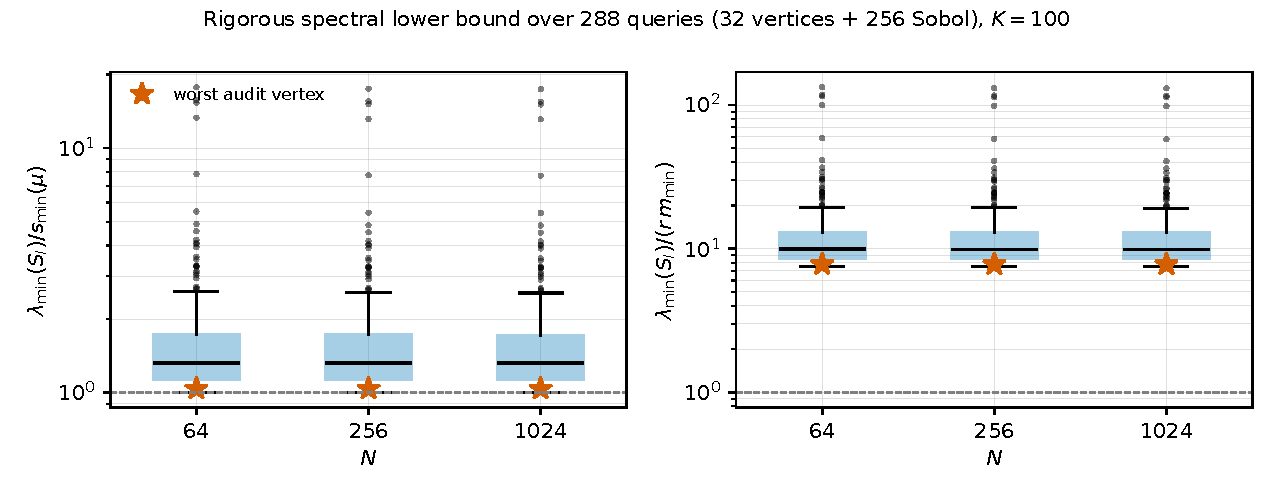
\includegraphics[width=0.94\linewidth]{F2_spectral_bound.pdf}
\caption{Ratios $\lambda_{\min}(S_I)/\smin(\mu)$ (left) and $\lambda_{\min}(S_I)/(\rf m_{\min})$ (right)
over the 288 verification queries at $N=64,256,1024$; the star marks the vertex
$\mu=(0.05,5,9,1.1,0.01)$, at which $\lambda_{\min}(S_I)/\smin(\mu)$ is closest to one.  Both ratios are $\ge1$ at every query, as Theorem~\ref{thm:spectral} asserts.}
\label{fig:spectral-bound}
\end{figure}
\begin{figure}[!htbp]
\centering
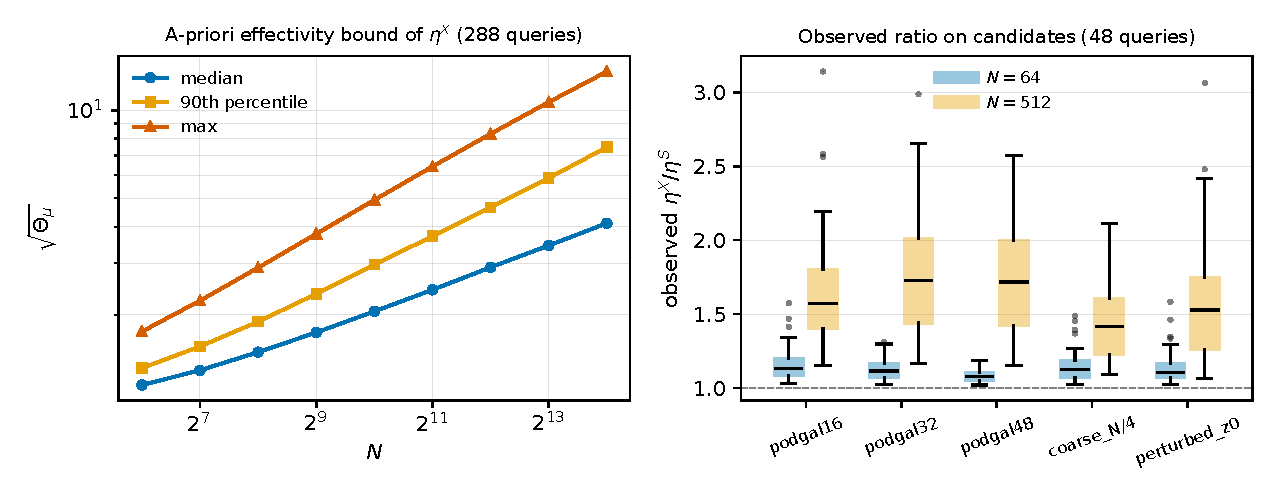
\includegraphics[width=0.94\linewidth]{F3_theta_and_effectivity.pdf}
\caption{Left: the a-priori effectivity bound $\sqrt{\Thmu}$ of the banded certificate as a function of
$N$ (symbol only, 288 queries).  Right: observed ratio $\eta^X/\eta^S$ for POD--Galerkin candidates
(ranks 16, 32, 48), the prolonged coarse solution and exact dynamics from a perturbed initial vector,
at $N=64$ and $N=512$.}
\label{fig:theta}
\end{figure}
The bound of Theorem~\ref{thm:spectral} and the two-sided comparison \eqref{eq:comparison} hold at
all $289\times3$ tested (query, $N$) pairs (the 288 verification queries and the starred vertex); the generalised eigenvalues of $(S_I,X_I)$ lie in
$[1,\Thmu]$ in every case.  The a-priori factor $\sqrt{\Thmu}$ grows like
$(\min(G,M)h)^{(Y-2)/2}$ (median $1.15$, $1.74$, $2.05$, $2.91$, $4.11$ at $N=64$, $512$, $1024$,
$4096$, $16384$; maxima $1.75$, $3.78$, $4.93$, $8.30$, $13.6$), because the tempering scale moves
below the resolution of a degree-$(p-1)$ trigonometric minorant.  The observed ratio
$\eta^X/\eta^S$ on candidates is much smaller: median $1.08$--$1.13$ at $N=64$ and $1.4$--$1.7$ at
$N=512$ (maximum $3.1$), so at the production resolution the banded certificate costs a factor
below two in effectivity; the production candidates of Section~\ref{ssec:e1} confirm the factor
$\eta^X/\eta^S\approx2$ at $N=1024$.
\subsection{Riesz solves and reference trajectories}
\begin{table}[!htbp]
\centering\small
\caption{Iteration counts (median / max over 20 Sobol queries) to relative residual $10^{-12}$: conjugate gradients for the Riesz system $S_Iv=\rho$ with and without the circulant preconditioner built from the symbol samples, and circulant-preconditioned GMRES per Crank--Nicolson step for $B_+=M_I+\tfrac{\Delta\tau}{2}A_I$ (60 steps, warm start, mean over steps / max).}
\label{tab:pcg-v9}
\begin{tabular}{rrrr}
\toprule
$N$ & plain CG & circulant PCG & circulant GMRES ($B_+$)\\
\midrule
64 & 42 / 45 & 8 / 8 & 5.0 / 5\\
128 & 74 / 82 & 9 / 9 & 5.0 / 6\\
256 & 130 / 154 & 9 / 10 & 6.0 / 7\\
512 & 224 / 292 & 10 / 10 & 7.0 / 8\\
1024 & 384 / 548 & 10 / 11 & 7.1 / 12\\
2048 & 648 / 1025 & 11 / 11 & 8.0 / 13\\
4096 & 1080 / 1915 & 11 / 12 & 9.0 / 15\\
\bottomrule
\end{tabular}
\end{table}

Dense-LU and circulant-GMRES references agree to $10^{-12}$ in the $M_I$ norm for
$N\le1024$; the bracket width at convergence is below $10^{-20}$ relative for $N\le1024$ and
below $10^{-18}$ at $N=4096$, where it is set by the roundoff of the recomputed residual.
\subsection{Initial-error tests and \texorpdfstring{$Y<1$}{Y<1}}
On the 48 exact-dynamics cases with perturbed initial vectors ($\|\delta\|_{M_I}=10^{-4}$), both
$\eta^X_{\rm aug}$ and $\eta^S_{\rm aug}$ hold with effectivity $1.00\pm10^{-6}$, whereas the
residual-only estimators (without $\beta_0$) underestimate the error in every case, which confirms
that the initial term of the augmented bound is essential.  For $Y\in\{0.5,0.8,0.95\}$
(same $C,G,M,\rf$ as the reference query) the bound $\alpha_{\rm lb}=0.0500=\rf$ is positive,
$\lambda_{\min}(S_I)\in[0.052,0.055]$, $\sqrt{\Thmu}\le1.5$, the preconditioned GMRES solve of
$B_+$ needs at most five iterations per step, and the certificate holds with effectivity one on
perturbed exact dynamics; the discrete framework therefore covers the finite-variation regime
without change.
\section{Stress test: a neural operator trained on a different discretisation}
\label{sm:deeponet}
The neural-operator candidate is a DeepONet with payoff and parameter branches and a time
trunk, latent dimension 64 and 80,002 trainable parameters, followed by a coefficient decoder
that supplies the spline-valued output; with $\mathcal K=100$ fixed it is a parameter map for a
single strike, and the payoff branch accommodates other payoffs.  It is trained on the
principal-period ($K=0$) discretisation, which differs from the exact Galerkin system by
$0.31$--$0.41$ in relative operator norm (Table~\ref{tab:assembly-v9}), and is certified as a
candidate of the exact system ($N=64$, $N_T=60$, 120 benchmark queries).  The certificate rejects it
at every tolerance of the sweep $10^{-3}\times\{0.1,\dots,10\}$: the median true error is $0.78$
(relative $3.1\times10^{-3}$), the median exact bound $3.4$, with no false accept.  The certificate
thus detects, query by query, that a surrogate was trained for a different discrete problem; the
neural candidate of the production study is the POD-NN below.
\section{Neural reduced candidates: results and training details}
\label{sm:training}
Table~\ref{tab:podnn} reports every POD-NN checkpoint of Section~\ref{ssec:e1} of the main text on
the 30 validation queries, and Table~\ref{tab:training} lists the optimiser, schedule, parameter
counts and wall times of the runs.
\begin{table}[!htbp]
\centering\small
\caption{Neural reduced candidates (POD-NN, $r=48$) on the 30 validation queries at the production configuration: median true error and median augmented bounds of the three certificates, with the effectivity of the exact one. Standard output: $r\times N_T$ coefficients; space--time output: $r\times r_t$ coefficients of a temporal POD ($r_t=23$). Checkpoints selected by the validation median of the reduced certificate. The projection of the reference trajectories onto the same basis and the POD--Galerkin solution are the attainable floor. At $\varepsilon_N=1.18\times10^{-3}$ the certificate rejects every POD-NN query, each by the cheap rejection of the first stage.}
\label{tab:podnn}
\resizebox{\textwidth}{!}{%
\begin{tabular}{lrrrrr}
\toprule
candidate & error & $\eta^S_{\rm aug}$ & $\eta^X_{\rm aug}$ & $\eta^{\bar X}_{\rm aug}$ & eff.\ $\eta^S$\\
\midrule
800 traj., $\lambda_R=0$ & 0.183 & 33.7 & 42.0 & 103 & 178.5\\
800 traj., $\lambda_R=1$ & 1.76 & 5.20 & 8.19 & 18.9 & 3.0\\
4000 traj., $\lambda_R=0$ & 0.0816 & 12.2 & 16.4 & 37.4 & 148.0\\
4000 traj., $\lambda_R=10^{-2}$ & 0.448 & 1.27 & 2.11 & 4.90 & 2.9\\
4000 traj., $\lambda_R=10^{-1}$ & 0.485 & 1.28 & 2.15 & 4.95 & 2.8\\
4000 traj., $\lambda_R=1$, seed 0 & 0.458 & 1.26 & 2.07 & 4.94 & 2.9\\
\quad seed 1 & 0.473 & 1.24 & 2.04 & 4.80 & 2.8\\
\quad seed 2 & 0.464 & 1.27 & 2.08 & 4.95 & 2.8\\
space--time, 4000 traj., $\lambda_R=1$, seed 0 & 0.0159 & 0.0582 & 0.0891 & 0.190 & 3.7\\
\quad seed 1 & 0.0161 & 0.0559 & 0.0841 & 0.195 & 3.6\\
\quad seed 2 & 0.0142 & 0.0545 & 0.0815 & 0.176 & 3.8\\
\midrule
projection of the references & $3.3\times10^{-4}$ & $3.2\times10^{-3}$ & $6.2\times10^{-3}$ & 0.0127 & 10.2\\
POD--Galerkin, $r=48$ & $3.5\times10^{-4}$ & $3.8\times10^{-3}$ & $8.2\times10^{-3}$ & 0.0154 & 11.0\\
\bottomrule
\end{tabular}}
\end{table}

\begin{table}[!htbp]
\centering\small
\caption{POD-NN training details (production configuration). MLP $6\to256\to256\to256\to$ output with SiLU, double precision, inputs $(\mu,T)$ standardised, $\alpha^0$ fixed to the projection of $z_h^0$; loss = relative least squares in the reduced coordinates $+\lambda_R\,\eta^{\bar X}$ (reduced online certificate, differentiable); Adam, learning rate $10^{-3}$ with cosine decay to $10^{-5}$, 2000 epochs, batch 64, validation every 10 epochs on the 30-query set, checkpoint = epoch with the smallest median reduced bound. Intel Core Ultra 9 285K, 3 threads per run.}
\label{tab:training}
\resizebox{\textwidth}{!}{%
\begin{tabular}{lrrrr}
\toprule
variant & output & parameters & runs & wall time per run (h)\\
\midrule
standard, 800 trajectories & $r\times N_T=11\,520$ & $3.09$~M & $\lambda_R\in\{0,10^{-2},10^{-1},1\}$, seed 0 & 0.9--2.7\\
standard, 4000 trajectories & $r\times N_T=11\,520$ & $3.09$~M & $\lambda_R\in\{0,10^{-2},10^{-1},1\}$, seed 0; $\lambda_R=1$, seeds 1--2 & 3.5--7.8\\
space--time, 4000 trajectories & $r\times r_t=1\,104$ & $0.42$~M & $\lambda_R=1$, seeds 0--2 & 5.9--7.1\\
\bottomrule
\end{tabular}}
\end{table}

\section{Operation counts and measured constants of the cost model}
\label{sm:cost}
Let ${\rm it}_B$ be the mean number of preconditioned GMRES iterations per Crank--Nicolson step
(Table~\ref{tab:pcg-v9}: $5$--$9$), and count one FFT of length $2N_h$ as $5N_h\log_2N_h$
flops.  Per query,
\begin{align*}
 \text{direct solve:}&\quad N_T\,{\rm it}_B\,(2\cdot5N_h\log_2N_h+O(N_h)),\\
 \text{certificate }(\eta^X):&\quad N_T\,(2\cdot5N_h\log_2N_h)+N_T(2p-1)N_h+O(p^2N_h),\\
 \text{certificate }(\eta^S):&\quad N_T\,{\rm it}_{\rm PCG}\,(2\cdot5N_h\log_2N_h)+\text{the above},\\
 \text{reduced solve:}&\quad (Q+2)r^2+N_T\,r^2,\\
 \text{reduced certificate }(\eta^{\bar X}):&\quad \varrho\,(Q+2)(2r+1)+N_T\,r\,(Q+2),
\end{align*}
with $\varrho\le N_h$ retained rows, plus the symbol evaluation $O(LK)$ common to all certified variants.  These counts underlie Section~\ref{ssec:cost} of the main text;
Table~\ref{tab:cost} gives the measured constants from the refinement study of
Section~\ref{ssec:benchmark}.
\begin{table}[!htbp]
\centering\small
\caption{Cost model of Section~\ref{ssec:cost} with measured constants (one thread, idle machine; medians over five benchmark queries; $m=2N_h$, $i_n$ and $p_n$ the GMRES and PCG iteration counts per step). Times in ms; $c$ is the fitted time per operation of the stated count with its maximum relative deviation; where the per-step interpreter overhead matters the two-constant fit $t=c'\,\mathrm{ops}+d\,\mathrm{calls}$ is also given. The spectral-data row is the fine verification grid; the online path uses the fast mode ($2.5$~ms, Section~\ref{ssec:benchmark}). The reduced rows do not depend on $N$ by construction.}
\label{tab:cost}
\resizebox{\textwidth}{!}{%
\begin{tabular}{lrrrrrrr}
\toprule
component & op count & $N=256$ & $N=512$ & $N=1024$ & $N=2048$ & $N=4096$ & $c$ (fit res.)\\
\midrule
assembly & $L(2K+1)$ & 21.63 & 57.02 & 106.37 & 209.78 & 408.07 & $1.25\times10^{-7}$ (16\%)\\
spectral data (fine mode; online fast mode $2.5$~ms) & $n_g(2K+1)$ & 477.85 & 478.78 & 476.70 & 476.52 & 476.85 & $1.23\times10^{-7}$ (1\%)\\
direct solve & $(\sum_n i_n+N_T)\,m\log m$ & 76.64 & 78.41 & 148.17 & 246.94 & 591.73 & $4.52\times10^{-9}$ (156\%); $c'=2.2\times10^{-9}$, $d=3.7\times10^{-5}$ (11\%)\\
residual & $N_T\,m\log m$ & 1.11 & 2.47 & 6.18 & 15.27 & 53.96 & $1.25\times10^{-9}$ (68\%)\\
banded $\eta^X$ & $N_T N_h$ & 0.80 & 1.61 & 3.33 & 6.76 & 13.38 & $1.35\times10^{-8}$ (6\%); $c'=1.3\times10^{-8}$, $d=0$ (6\%)\\
exact $\eta^S$ & $\sum_n p_n\,m\log m$ & 61.49 & 60.83 & 141.40 & 237.32 & 678.46 & $2.65\times10^{-9}$ (115\%); $c'=1.7\times10^{-9}$, $d=1.2\times10^{-5}$ (21\%)\\
\midrule
\multicolumn{8}{l}{reduced model at $N=1024$, $Q=36$ (independent of $N$ by construction)}\\
component & op count & $r=16$ & $r=32$ & $r=48$ & $r=64$ & $r=80$ & $c$ (fit res.)\\
reduced solve & $(Q{+}2)r^2+r^3+3N_Tr^2$ & 0.78 & 0.86 & 0.97 & 1.11 & 1.29 & $5.37\times10^{-10}$ (638\%); $c'=8.8\times10^{-11}$, $d=3.3\times10^{-6}$ (4\%)\\
reduced certificate & $\rho(r{+}1)(Q{+}2{+}2N_T)$ & 0.27 & 0.61 & 1.10 & 1.80 & 2.74 & $8.73\times10^{-11}$ (36\%); $c'=7.6\times10^{-11}$, $d=3.9\times10^{-7}$ (4\%)\\
$\ell(\nu)+\varepsilon_Q$ & $161(2K+1)$ & 2.73 & 2.73 & 2.73 & 2.73 & 2.73 & $8.56\times10^{-8}$ (3\%)\\
$\rho$ (retained rows) & & 263 & 390 & 524 & 668 & 819 & \\
\bottomrule
\end{tabular}}
\end{table}

\FloatBarrier
\section{Extensions not used in the main text}
\label{sm:extensions}
The following results complement the main article; none of its statements depends on them.
\subsection{Discrete parameter stability}
\label{ssec:solution-operator}
\begin{proposition}[Discrete parameter stability of the solution map]
\label{prop:discrete-lipschitz}
Fix a mesh, a time grid, and a payoff $\psi$; the assembled symmetric
matrix $\Sh(\mu_1)$ is positive definite by Theorem~\ref{thm:spectral}. Let
$\mu_1,\mu_2\in\Pset$
with $\cc_h(\mu_1),\cc_h(\mu_2)$ the corresponding Crank--Nicolson
trajectories of \eqref{eq:cn-reference}.  Then, for every
$m=1,\dots,N_T$,
\begin{equation}
\begin{aligned}
  \norm{\cc_h^m(\mu_1)-\cc_h^m(\mu_2)}_{\Mh}^2
  \le{}& \norm{\cc_h^0(\mu_1)-\cc_h^0(\mu_2)}_{\Mh}^2\\
  &+\dt\sum_{n=0}^{m-1}
  \bigl\lVert\bm\varrho^{\,n+1/2}\bigr\rVert_{\Sh(\mu_1)^{-1}}^2 ,
\end{aligned}
  \label{eq:discrete-lipschitz}
\end{equation}
where the parameter-perturbation residual is
\begin{equation}
  \bm\varrho^{\,n+1/2}
  :=\bigl(\Ah(\mu_1)-\Ah(\mu_2)\bigr)\overline\cc_h^{\,n+1/2}(\mu_2)
   -\bigl(\overline\ff^{\,n+1/2}(\mu_1)-\overline\ff^{\,n+1/2}(\mu_2)\bigr).
  \label{eq:param-residual}
\end{equation}
Under exact assembly of the conforming variational matrices,
Theorem~\ref{thm:uniform-coercivity} additionally gives
\begin{equation}
\begin{aligned}
  &\norm{\bigl(\Ah(\mu_1)-\Ah(\mu_2)\bigr)\vv}_{\Sh(\mu_1)^{-1}}\\
  &\qquad\le
  \frac{1}{c_1}\,
  \sup_{0\ne v_h,w_h\in\Vh}
  \frac{|a_{\mu_1}(v_h,w_h)-a_{\mu_2}(v_h,w_h)|}
       {\norm{v_h}_{\Vp{\mu_1}}\norm{w_h}_{\Vp{\mu_1}}}\,
  \norm{\vv}_{\Sh(\mu_1)},
\end{aligned}
  \label{eq:matrix-difference}
\end{equation}
so a bound on the difference of the two bilinear forms in a \emph{single}
norm---that of $\mu_1$---suffices, and no common energy space is needed.
\end{proposition}

\begin{proof}
The difference $\ee^n:=\cc_h^n(\mu_1)-\cc_h^n(\mu_2)$ satisfies the
Crank--Nicolson error equation \eqref{eq:discrete-error-equation} with
$\rr_\theta^{n+1/2}$ replaced by $\bm\varrho^{\,n+1/2}$ of
\eqref{eq:param-residual}, since $\cc_h(\mu_2)$ solves the $\mu_2$ scheme
exactly.  Apply Theorem~\ref{thm:fully-discrete-certificate} with
$\Sh=\Sh(\mu_1)$.  Estimate \eqref{eq:matrix-difference} follows from
the continuity argument above applied to the bilinear form
$a_{\mu_1}-a_{\mu_2}$.
\end{proof}
This fixed-grid statement compares both trajectories in the norm of the
first parameter.

\subsection{Other time schemes and exponential shifts}
\label{ssec:semidiscrete}\label{ssec:be-certificate}\label{ssec:shifted}
The following extensions follow the same energy argument as
Theorem~\ref{thm:fully-discrete-certificate}.
For a differentiable candidate and a semidiscrete reference, define
$\rho=\Mh\dot\cc_\theta+\Ah\cc_\theta-\ff$. Then
\begin{equation}
 \|\ee(t)\|_{\Mh}^2+\int_0^t\|\ee\|_{\Sh}^2
 \le\|\ee(0)\|_{\Mh}^2+\int_0^t\|\rho\|_{\Sh^{-1}}^2.
 \label{eq:semidiscrete-certificate}
\end{equation}
Multiply the error equation by $\ee^\top$, apply Young's inequality, and
integrate.
For backward Euler, the residual is
$\rho^{n+1}=\Mh(c_\theta^{n+1}-c_\theta^n)/\dt_n
+\Ah c_\theta^{n+1}-f^{n+1}$ and
\begin{equation}
 \|\ee^{n+1}\|_{\Mh}^2+\|\ee^{n+1}-\ee^n\|_{\Mh}^2
 +\dt_n\|\ee^{n+1}\|_{\Sh}^2
 \le\|\ee^n\|_{\Mh}^2+\dt_n\|\rho^{n+1}\|_{\Sh^{-1}}^2.
 \label{eq:be-certificate}
\end{equation}
This follows from
$2y^\top\Mh(y-z)=\|y\|_{\Mh}^2-\|z\|_{\Mh}^2+\|y-z\|_{\Mh}^2$.
A Rannacher start combines backward-Euler half steps with CN
\cite{Rannacher1984}; summing the corresponding bounds, with the initial
term retained, gives the certificate for the mixed trajectory.
Each step must use its own scheme's residual.

For an exact-assembly G\aa rding bound
$a_\mu(v,v)\ge c_1\|v\|_{V_\mu}^2-c_2\|v\|_{L^2}^2$, choose
$\sigma>c_2$ and set
$A_\sigma=\Ah+\sigma\Mh$, $S_\sigma=\Sh+\sigma\Mh$.
Then $S_\sigma\succeq(\sigma-c_2)\Mh$.
Advance $d_h$ by CN for the shifted operator with forcing
$g^n=e^{-\sigma\tau_n}f^n$, and reconstruct
$c_{h,\sigma}^n=e^{\sigma\tau_n}d_h^n$.
For $d_\theta^n=e^{-\sigma\tau_n}c_\theta^n$ and its shifted CN residual
$\rho_\sigma$, the same theorem yields
\[
 \max_m\|c_{h,\sigma}^m-c_\theta^m\|_{\Mh}
 \le e^{\sigma T}
 \left(\|d_h^0-d_\theta^0\|_{\Mh}^2+
 \dt\sum_n\|\rho_\sigma^{n+1/2}\|_{S_\sigma^{-1}}^2\right)^{1/2}.
\]
This certifies the reconstructed shifted target, which is a discrete trajectory
distinct from unshifted CN because exponential transformation and CN
discretisation do not commute. With positive rates no shift is needed, and the
numerical studies use unshifted CN.

\subsection{Preconditioned correction}
\label{ssec:correction-extension}
If $P_h\succ0$ and $\Sh\succeq\gamma_P P_h$ with $\gamma_P>0$, then
$r^\top\Sh^{-1}r\le\gamma_P^{-1}r^\top P_h^{-1}r$.
Alternatively $P_h$ can accelerate the Riesz iteration while the bracket
uses its independent bound on $\lambda_{\min}(\Sh)$.
\begin{proposition}[Contraction of a preconditioned correction]
\label{prop:correction-contraction}
Fix a time step and write the step equation as $B_+\zz=\bb$.  Let $P\succ0$ be
a preconditioner and consider the Richardson iteration
$\zz^{(i+1)}=\zz^{(i)}+P^{-1}(\bb-B_+\zz^{(i)})$ with residuals
$\sres^{(i)}=\bb-B_+\zz^{(i)}$.  Then
\begin{equation}
  \norm{\sres^{(i+1)}}_{P^{-1}}\le\rho_P\,\norm{\sres^{(i)}}_{P^{-1}},
  \qquad
  \rho_P:=\bigl\lVert I-P^{-1/2}B_+P^{-1/2}\bigr\rVert_2 .
  \label{eq:contraction}
\end{equation}
If $P=\Mh+\tfrac{\dt}{2}\Sh$, the symmetric part of $B_+$, then
\[
I-P^{-1/2}B_+P^{-1/2}=-\tfrac{\dt}{2}P^{-1/2}N_hP^{-1/2},\qquad N_h=\tfrac12(\Ah-\Ah^\top),
\]
with $N_h$ skew symmetric, so $\rho_P$ is determined entirely by the nonsymmetric part of the
CGMY operator and satisfies $\rho_P\le\tfrac{\dt}{2}\lVert P^{-1/2}N_hP^{-1/2}\rVert_2$.
\end{proposition}

\begin{proof}
$\sres^{(i+1)}=(I-B_+P^{-1})\sres^{(i)}$, so
$P^{-1/2}\sres^{(i+1)}=(I-P^{-1/2}B_+P^{-1/2})P^{-1/2}\sres^{(i)}$ and
\eqref{eq:contraction} follows by taking Euclidean norms.  For the second
claim, $B_+=P+\tfrac{\dt}{2}N_h$ by \eqref{eq:Sh} and the definition of $N_h$.
\end{proof}
The Richardson correction therefore contracts whenever $\rho_P<1$, a condition
governed by the skew part of the operator and the step size.  The experiments use
circulant-preconditioned GMRES, whose iteration counts are reported in Table~\ref{tab:pcg-v9}.
\begin{thebibliography}{99}
\bibitem{BarraultMadayNguyenPatera2004}
M. Barrault, Y. Maday, N.~C. Nguyen and A.~T. Patera, \emph{An `empirical interpolation' method:
application to efficient reduced-basis discretization of partial differential equations},
C. R. Math. Acad. Sci. Paris 339 (2004), 667--672.

\bibitem{BhattacharyaEtAl2021}
K.~Bhattacharya, B.~Hosseini, N.~B. Kovachki, and A.~M. Stuart,
\newblock Model reduction and neural networks for parametric PDEs,
\newblock \emph{SMAI Journal of Computational Mathematics}, 7 (2021),
pp.~121--157.

\bibitem{BottcherSilbermann1999}
A. B\"ottcher and B. Silbermann, \emph{Introduction to Large Truncated Toeplitz Matrices}, Springer, 1999.

\bibitem{BuhrEngwerOhlbergerRave2014}
A. Buhr, C. Engwer, M. Ohlberger and S. Rave, \emph{A numerically stable a posteriori error
estimator for reduced basis approximations of elliptic equations}, in: Proc. WCCM XI, 2014.

\bibitem{BurkovskaHaasdonkSalomonWohlmuth2015}
O. Burkovska, B. Haasdonk, J. Salomon and B. Wohlmuth, \emph{Reduced basis methods for pricing
options with the Black--Scholes and Heston models}, SIAM J. Financial Math. 6 (2015), 685--712.

\bibitem{CarrGemanMadanYor2002}
P.~Carr, H.~Geman, D.~B. Madan, and M.~Yor,
\newblock The fine structure of asset returns: an empirical investigation,
\newblock \emph{Journal of Business}, 75 (2002), pp.~305--332.

\bibitem{CarteadelCastilloNegrete2007}
\'A.~Cartea and D.~del Castillo-Negrete,
\newblock Fractional diffusion models of option prices in markets with jumps,
\newblock \emph{Physica A}, 374 (2007), pp.~749--763.

\bibitem{CasenaveErnLelievre2014}
F. Casenave, A. Ern and T. Leli\`evre, \emph{Accurate and online-efficient evaluation of the a
posteriori error bound in the reduced basis method}, M2AN 48 (2014), 207--229.

\bibitem{ChanStrang1989}
R.~H. Chan and G. Strang, \emph{Toeplitz equations by conjugate gradients with circulant
preconditioner}, SIAM J. Sci. Statist. Comput. 10 (1989), 104--119.

\bibitem{ContLantosPironneau2011}
R.~Cont, N.~Lantos, and O.~Pironneau,
\newblock A reduced basis for option pricing,
\newblock \emph{SIAM Journal on Financial Mathematics}, 2 (2011),
pp.~287--316. DOI: \url{https://doi.org/10.1137/10079851X}.

\bibitem{ContVoltchkova2005}
R.~Cont and E.~Voltchkova,
\newblock A finite difference scheme for option pricing in jump diffusion and
exponential L\'evy models,
\newblock \emph{SIAM Journal on Numerical Analysis}, 43 (2005),
pp.~1596--1626.

\bibitem{DamircheliCGMY2026}
D.~Damircheli,
\newblock A B-spline Galerkin method for option pricing under the CGMY
tempered stable process,
\newblock submitted to \emph{SIAM Journal on Financial Mathematics}, 2026.

\bibitem{FangOosterlee2008}
F.~Fang and C.~W. Oosterlee,
\newblock A novel pricing method for European options based on Fourier-cosine
series expansions,
\newblock \emph{SIAM Journal on Scientific Computing}, 31 (2008),
pp.~826--848.

\bibitem{GassGlauMahlstedtMair2018}
M. Gass, K. Glau, M. Mahlstedt and M. Mair, \emph{Chebyshev interpolation for parametric option
pricing}, Finance Stoch. 22 (2018), 701--731.

\bibitem{GrenanderSzego1958}
U. Grenander and G. Szeg\H{o}, \emph{Toeplitz Forms and Their Applications}, Univ. of California Press, 1958.

\bibitem{GreplMadayNguyenPatera2007}
M.~A. Grepl, Y. Maday, N.~C. Nguyen and A.~T. Patera, \emph{Efficient reduced-basis treatment of
nonaffine and nonlinear partial differential equations}, M2AN 41 (2007), 575--605.

\bibitem{GreplPatera2005}
M.~A. Grepl and A.~T. Patera,
\newblock A posteriori error bounds for reduced-basis approximations of
parametrized parabolic partial differential equations,
\newblock \emph{ESAIM: Mathematical Modelling and Numerical Analysis},
39 (2005), pp.~157--181.

\bibitem{HaasdonkOhlberger2008}
B.~Haasdonk and M.~Ohlberger,
\newblock Reduced basis method for finite volume approximations of
parametrized linear evolution equations,
\newblock \emph{ESAIM: Mathematical Modelling and Numerical Analysis},
42 (2008), pp.~277--302.

\bibitem{HesthavenUbbiali2018}
J.~S. Hesthaven and S.~Ubbiali,
\newblock Non-intrusive reduced order modeling of nonlinear problems using
neural networks,
\newblock \emph{Journal of Computational Physics}, 363 (2018), pp.~55--78.

\bibitem{HilberReichmannSchwabWinter2013}
N.~Hilber, O.~Reichmann, C.~Schwab, and C.~Winter,
\newblock \emph{Computational Methods for Quantitative Finance: Finite Element
Methods for Derivative Pricing},
\newblock Springer, Berlin, 2013.

\bibitem{HuynhRozzaSenPatera2007}
D.~B.~P. Huynh, G. Rozza, S. Sen and A.~T. Patera, \emph{A successive constraint linear optimization
method for lower bounds of parametric coercivity and inf-sup stability constants},
C. R. Math. Acad. Sci. Paris 345 (2007), 473--478.

\bibitem{KovachkiEtAl2023}
N.~Kovachki, Z.~Li, B.~Liu, K.~Azizzadenesheli, K.~Bhattacharya, A.~Stuart,
and A.~Anandkumar,
\newblock Neural operator: learning maps between function spaces with
applications to PDEs,
\newblock \emph{Journal of Machine Learning Research}, 24 (2023), pp.~1--97.

\bibitem{LiKovachkiEtAl2021}
Z.~Li, N.~Kovachki, K.~Azizzadenesheli, B.~Liu, K.~Bhattacharya, A.~Stuart,
and A.~Anandkumar,
\newblock Fourier neural operator for parametric partial differential
equations,
\newblock International Conference on Learning Representations, 2021.

\bibitem{LuJinPangZhangKarniadakis2021}
L.~Lu, P.~Jin, G.~Pang, Z.~Zhang, and G.~E. Karniadakis,
\newblock Learning nonlinear operators via DeepONet based on the universal
approximation theorem of operators,
\newblock \emph{Nature Machine Intelligence}, 3 (2021), pp.~218--229.

\bibitem{MatacheVonPetersdorffSchwab2004}
A.-M. Matache, T.~von Petersdorff, and C.~Schwab,
\newblock Fast deterministic pricing of options on L\'evy driven assets,
\newblock \emph{ESAIM: Mathematical Modelling and Numerical Analysis},
38 (2004), pp.~37--71.

\bibitem{QiuDahmenChen2026}
Y.~Qiu, W.~Dahmen, and P.~Chen,
\newblock Variationally correct operator learning: reduced basis neural
operator with a posteriori error estimation,
\newblock \emph{Computer Methods in Applied Mechanics and Engineering},
461, Part B (2026), 119228.
DOI: \url{https://doi.org/10.1016/j.cma.2026.119228}.

\bibitem{Rannacher1984}
R.~Rannacher,
\newblock Finite element solution of diffusion problems with irregular data,
\newblock \emph{Numerische Mathematik}, 43 (1984), pp.~309--327.

\bibitem{RozzaHuynhPatera2008}
G.~Rozza, D.~B.~P. Huynh, and A.~T. Patera,
\newblock Reduced basis approximation and a posteriori error estimation for
affinely parametrized elliptic coercive partial differential equations,
\newblock \emph{Archives of Computational Methods in Engineering},
15 (2008), pp.~229--275.

\bibitem{YouYuDEliaGaoSilling2022}
H.~You, Y.~Yu, M.~D'Elia, T.~Gao, and S.~Silling,
\newblock Nonlocal kernel network (NKN): a stable and resolution-independent
deep neural network,
\newblock \emph{Journal of Computational Physics}, 469 (2022), 111536.

\end{thebibliography}

\end{document}
